\documentclass{beamer}
\usepackage{tikz-cd}
\usetheme{Boadilla}
\usepackage{wrapfig}

\title{Physics and the Absolute Conception}
\author{Hans Halvorson}
\institute{Princeton University}
\date{September 6, 2019}


\begin{document}

\begin{frame}
\titlepage
\end{frame}

\begin{frame}

  \begin{itemize}
  \item Physics is held up as the paradigm of objective knowledge
    \begin{enumerate}
    \item In public discourse
    \item In analytic metaphysics and ethics
    \end{enumerate}
  \item Objectivity should be a concretely implementable intellectual
    virtue
  \item Objectivity is a norm for choice of theory and/or research
    program
  \item Two pictures of objectivity
  \begin{enumerate} \item Einstein: absolute conception, god's eye view
  \item Bohr: unambiguous communication
  \end{enumerate}
\end{itemize}


\end{frame}

\begin{frame}
\frametitle{Outline}
\tableofcontents
\end{frame}

\section{Einstein's divine aspiration}

\begin{frame}

  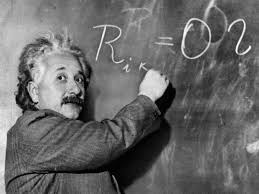
\includegraphics[scale=0.7]{einstein.jpeg}

  \bigskip ``I want to know God's thoughts, the rest are details.''

\end{frame}

%%%%%%%%%%%%%%%%%%%%%%%%%%%%%%

\begin{frame}
\frametitle{Bernard Williams: the absolute conception}

\begin{wrapfigure}{r}{2in} 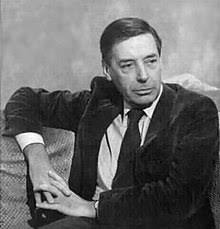
\includegraphics[scale=0.4]{williams.jpeg} \end{wrapfigure}

``What God has given us, according to Descartes, is an insight into
the nature of \underline{the world as it seems to God}, and the world
as it seems to God must be the world as it really is.''

\bigskip ``\ldots a conception of reality as it is
\underline{independently of our thought}, and to which all
representations of reality can be related.''

\bigskip ``\ldots there must be some coherent way of understanding why
these representations differ, and how they are related to one
another.''
\end{frame}

\begin{frame}
  \frametitle{North Atlantic Metaphysical Madness \\ theory without convention}

  \begin{tabular}{c c c}
    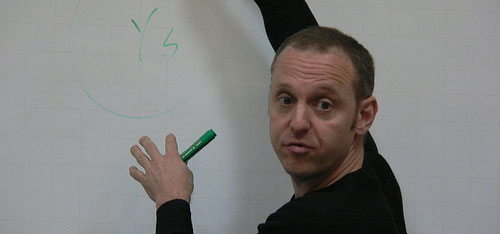
\includegraphics[scale=0.25]{sider.jpg} &
                                              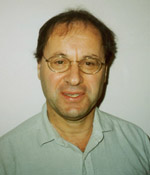
\includegraphics[scale=1.5]{find.jpg}
    & 
\includegraphics[scale=0.04]{williamson.jpg} \end{tabular}

  %% TO DO: pictures of Sider, Fine, Williamson

  %% TO DO: tikz picture with arrows

\bigskip
                                            
  \begin{tabular}{l l l l l}
    $T_1$ & & $\forall x\exists yRxy$  & & \\ \\
    $T_2$ & & $\forall y\exists xRxy$ \\ \\
    $T^+$ & & there is a serial relation \end{tabular}

  %% TO DO: picture of the common definitional extension


  \end{frame}
\begin{frame}
  \frametitle{coordinate free description}

%% affine space as CDE

\end{frame}

\begin{frame}
  \frametitle{science liberated from language}

  ``The semantic view of theories makes language irrelevant to the
  subject'' (Bas van Fraassen)

  \bigskip ``In our discussion, a model is not such an interpretation [i.e.,
  not an $\Sigma$-structure], matching statements to a set of objects
  which bear certain relations among themselves, but the set of
  objects itself.'' (Lisa Lloyd)

\bigskip   \[ \{ \{ a,b,\langle a,a\rangle \} , \{ \langle a,a\rangle \} \} \]
  
  %% Lisa Lloyd

 \end{frame}

\begin{frame}
\frametitle{Summary: the Einstein view of objectivity}
  
  \begin{enumerate}
  \item The absolute conception (Williams) / view from nowhere (Nagel)
    / god's eye view (Putnam)
  \item Theory without conventions
  \item Spacetime description without coordinates
  \item Theory without language
    \newline
    No need for coordinative definitions
    \item Perfectly natural properties and relations (Lewis, Sider)
    \newline
    Don't depend on our interests (as Nelson Goodman suggested)  
  \end{enumerate}
\end{frame}

\begin{frame}
\frametitle{Summary: why the Einstein view fails}  

In the limit, objective description would be:
  \begin{enumerate}
  \item empirically ambiguous (description without a describer)
  \item impossible in principle (speech without a language)
  \end{enumerate}

\bigskip And yet, objectivity is a concrete intellectual virtue
  
\medskip Proposal: objectivity adds form to truth, where the substance
is provided by our individual subjective perspectives

\medskip Proposal: objectivity is a virtue, and like other virtues,
one has to be wary about maximization


\end{frame}



\section{Bohr on objective description}

%% TO DO: separation between subject and object


\begin{frame}
  \frametitle{objectivity as univocity}

  %% TO DO: picture of Niels Bohr

  \begin{figure}[c] 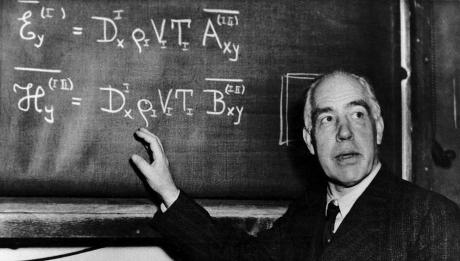
\includegraphics[scale=0.5]{bohr.jpg} \end{figure}

  \medskip Bohr ``Every scientist is constantly confronted with the
  problem of objective description of experience by which we mean
  \textbf{unambiguous communication}.''


  \bigskip Bohr: ``We must strive continually to extend the scope of
  our description, but in such a way that our messages do not thereby
  lose their \textbf{objective or unambiguous} character.''
\end{frame}

\begin{frame}
  \frametitle{objectivity as univocity}

  Bohr: ``\ldots the account of the experimental arrangement and of
  the results of the observations must be expressed in
  \textbf{unambiguous language} with suitable application of the
  terminology of classical physics.''

  \bigskip \bigskip Bohr: ``\ldots our task must be to account for
  such experience in a manner independent of individual subjective
  judgment and therefore objective in the sense that it can be
  \textbf{unambiguously communicated in ordinary human language}.''

\end{frame}

\begin{frame}
  \frametitle{objectivity via intertranslatability}

  Bohr: ``The relativistic description is also \textbf{objective}
  inasmuch as every observer can deduce by calculation what the other
  observer will perceive or has perceived.  For all that, we have come
  a long way from the classical ideal of objective descriptions.''

  \bigskip \bigskip $\Longrightarrow$ the formalism of relativity
  theory doesn't provide a system of subject-free truths, but a scheme
  for coordinating subject-relative truths

\end{frame}

\begin{frame}
  \frametitle{objectivity via intertranslatability}

  When are two first-order theories $T_1$ and $T_2$ equivalent?

  \begin{enumerate}
  \item (Montague) If the relation symbols of $T_1$ can be reinterpreted as
    relations in $T_2$, and the relation symbols of $T_2$ can be
    reinterpreted as relations in $T_1$ such that \dots
  \item (Morita) If the quantifier phrases of $T_1$ can be
    reinterpreted as \dots
  \end{enumerate}

  \bigskip \bigskip $\Longrightarrow$ we express how we understand our
  theories through the claims of equivalence we accept

  \medskip $\Longrightarrow$ we do \emph{not} base claims of
  equivalence on some theory (which is supposed not to require any
  interpretation)

\end{frame}  

\begin{frame}
  \frametitle{claims of equivalence between theories cannot be
    substantiated by a third theory}

  \begin{itemize}
  \item A third theory wouldn't help
      \begin{itemize}
      \item would be yet another competitor
      \item infinite regress of meta-questions
        \end{itemize}  
      \item We don't need a third theory
        \begin{itemize}
        \item we already have intuitions about equivalence
        \item empirical reality is our friend
        \end{itemize}
  \end{itemize}
  
\end{frame}


\begin{frame}
  \frametitle{Summary: what kind of objectivity can we aspire to?}

  \begin{enumerate}
  \item A good scientific theory enables coordination of diverse
    subjectivities
  \item Coordination is enabled by:
    \begin{enumerate} \item the existence of common experiential reference points 
      \item a subject's being able to make an object of itself \end{enumerate}
  \item We are ineliminably subjective 
  \end{enumerate}


\end{frame}



%%%
%%%
%%%

\section{Who is the realist about quantum theory?}

\begin{frame}
\frametitle{The old new story}
  
The Copenhagen interpretation of quantum theory is bad because it
involves ``observer'' or ``measurement'' as primitives.

\bigskip The many-worlds interpretation is good because it says what
the universe would be like, even if nobody was there to observe
it.

\end{frame}

\begin{frame}
  \frametitle{The new old story}

  The many-worlds interpretation is bad if it says nothing more than
  that the world is like some mathematical model.
  
  \bigskip \bigskip The Copenhagen interpretation is good because it
  gives rules that subjects can follow for using mathematical models
  to say true things about the concrete reality that they exist
  in. (cf. Richard Healey)

\end{frame}

\begin{frame}
  \frametitle{Lessons}
  \begin{enumerate}
  \item The search for the absolute conception is a fool's errand
  \item An absolute conception would be empirically ambiguous \newline
    ``The world is modelled by the number 42!''  \newline ``The world
    is a four-dimensional Lorentzian manifold!'' \newline ``The world
    is a wavefunction!''
  \item The phrase ``objective description'' is misleadingly used for
    a \emph{scheme} that coordinates various subjective viewpoints
  \item Such a scheme provides a description of reality only by means
    of a \emph{realization} in a subjective viewpoint
  \end{enumerate}
  \end{frame}

\end{document}




%%% Local Variables:
%%% mode: latex
%%% TeX-master: t
%%% End:
